\documentclass[11pt]{beamer}
\usepackage[utf8]{inputenc}
\usepackage{graphicx, epsfig}
\usepackage{amsmath,mathrsfs,amsfonts,amssymb}
%\usepackage{subfig}
\usepackage{floatflt}
\usepackage{epic,ecltree}
\usepackage{mathtext}
\usepackage{fancybox}
\usepackage{fancyhdr}
\usepackage{multirow}
\usepackage{enumerate}
\usepackage{epstopdf}
\usepackage{multicol}
\usepackage{algorithm}
\usepackage[noend]{algorithmic}
\usepackage{tikz}
\usepackage{blindtext}
\usetheme{default}%{default}%{Singapore}%{Warsaw}%{Warsaw}%{Darmstadt}
\usecolortheme{default}
\setbeamerfont{title}{size=\Huge}
\setbeamertemplate{footline}[page number]{}


\makeatletter
\newcommand\HUGE{\@setfontsize\Huge{35}{40}}
\makeatother    

\setbeamerfont{title}{size=\HUGE}
\beamertemplatenavigationsymbolsempty

% latin bold lower
\newcommand{\ba}{\mathbf{a}} 
\newcommand{\bc}{\mathbf{c}} 
\newcommand{\be}{\mathbf{e}} 
\newcommand{\bh}{\mathbf{h}} 
\newcommand{\bp}{\mathbf{p}} 
\newcommand{\bt}{\mathbf{t}} 
\newcommand{\bs}{\mathbf{s}} 
\newcommand{\bu}{\mathbf{u}} 
\newcommand{\bv}{\mathbf{v}} 
\newcommand{\bw}{\mathbf{w}} 
\newcommand{\bx}{\mathbf{x}} 
\newcommand{\by}{\mathbf{y}} 
\newcommand{\bz}{\mathbf{z}} 

% latin bold upper
\newcommand{\bA}{\mathbf{A}} 
\newcommand{\bB}{\mathbf{B}} 
\newcommand{\bC}{\mathbf{C}} 
\newcommand{\bI}{\mathbf{I}} 
\newcommand{\bL}{\mathbf{L}} 
\newcommand{\bM}{\mathbf{M}} 
\newcommand{\bQ}{\mathbf{Q}} 
\newcommand{\bT}{\mathbf{T}} 
\newcommand{\bU}{\mathbf{U}} 
\newcommand{\bV}{\mathbf{V}} 
\newcommand{\bW}{\mathbf{W}} 
\newcommand{\bX}{\mathbf{X}} 
\newcommand{\bY}{\mathbf{Y}} 
\newcommand{\bZ}{\mathbf{Z}} 

% latin cal upper
\newcommand{\cG}{\mathcal{G}} 
\newcommand{\cL}{\mathcal{L}} 
\newcommand{\cN}{\mathcal{N}} 
\newcommand{\cS}{\mathcal{S}} 
\newcommand{\cT}{\mathcal{T}} 
\newcommand{\cW}{\mathcal{W}} 
\newcommand{\cX}{\mathcal{X}} 
\newcommand{\cZ}{\mathcal{Z}} 

% latin bb upper
\newcommand{\bbE}{\mathbb{E}} 
\newcommand{\bbI}{\mathbb{I}} 
\newcommand{\bbP}{\mathbb{P}} 
\newcommand{\bbR}{\mathbb{R}} 

% greek bold lower
\newcommand{\bepsilon}{\boldsymbol{\epsilon}} 
\newcommand{\btheta}{\boldsymbol{\theta}} 
\newcommand{\blambda}{\boldsymbol{\lambda}} 
\newcommand{\bpi}{\boldsymbol{\pi}} 
\newcommand{\bmu}{\boldsymbol{\mu}} 
\newcommand{\bsigma}{\boldsymbol{\sigma}} 
\newcommand{\bphi}{\boldsymbol{\phi}} 

% greek bold upper
\newcommand{\bSigma}{\boldsymbol{\Sigma}} 

\DeclareMathOperator*{\argmin}{arg\,min}
\DeclareMathOperator*{\argmax}{arg\,max}
\newcommand{\createdgmtitle}[1]{\title[\hbox to 56mm{Mathematical Forecasting Methods \hfill\insertframenumber\,/\,\inserttotalframenumber}]
	{\vspace{1.5\cm} \\ Mathematical Forecasting Methods \\ {\Huge Лекция #1}}
	\author{}
	\institute{
	МФТИ
	} 
	\date{Осень, 2023}
}

\newcommand\myfootnote[1]{%
  \tikz[remember picture,overlay]
  \draw (current page.south west) +(1in + \oddsidemargin,0.5em)
  node[anchor=south west,inner sep=0pt]{\parbox{\textwidth}{%
      \rlap{\rule{10em}{0.4pt}}\raggedright\scriptsize \textit{#1}}};}

\newcommand\myfootnotewithlink[2]{%
  \tikz[remember picture,overlay]
  \draw (current page.south west) +(1in + \oddsidemargin,0.5em)
  node[anchor=south west,inner sep=0pt]{\parbox{\textwidth}{%
      \rlap{\rule{10em}{0.4pt}}\raggedright\scriptsize\href{#1}{\textit{#2}}}};}
\createdgmtitle{13}
\usepackage{tikz}
\usepackage{amsmath}
\usepackage[english,russian]{babel}
\usepackage[labelformat=empty]{caption}

\usepackage{graphicx,animate}
\usepackage{animate}
\usepackage{svg}
\usepackage{subcaption}

\usepackage{ stmaryrd }

\usetikzlibrary{arrows,shapes,positioning,shadows,trees}
\newcommand*{\defeq}{\stackrel{\text{def}}{=}}
\newcommand{\tensor}[1]{\underline{\textbf{#1}}}
\newcommand{\M}[1]{\textbf{#1}}
\newcommand{\norm}[1]{\lVert #1 \rVert }
%--------------------------------------------------------------------------------
\begin{document}
%--------------------------------------------------------------------------------
\begin{frame}[plain]
%\thispagestyle{empty}
\titlepage
\end{frame}
%=======
\begin{frame}{Краткое повторение: SVD}
Для аналогии вспомним разложение в случае матриц.\\
Любая матрица $\M{X} \in \mathbb{R}^{m \times n}$ представима в виде

$$ \M{X}
    = \M{U} \Sigma \M{V}^{\intercal}
    = \Sigma \times_1 \M{U} \times_2 \M{V}
    = \llbracket \Sigma; \M{U}, \M{V}\rrbracket
$$
Здесь:
\begin{itemize}
    \item Матрицы $\M{U} \in \mathbb{R}^{m \times m}$, $\M{V} \in \mathbb{R}^{n \times n}$ - ортогональные матрицы
    \item $ \Sigma = \text{diag}(\sigma_1,...,\sigma_{min(m,n)}) \in  \mathbb{R}^{m \times n}$ --- диагональная матрица сингулярных чисел,
    где $\sigma_1\geq ... \geq \sigma_{\min (m,n)}\geq 0$
\end{itemize}
\begin{figure}
    \centering
    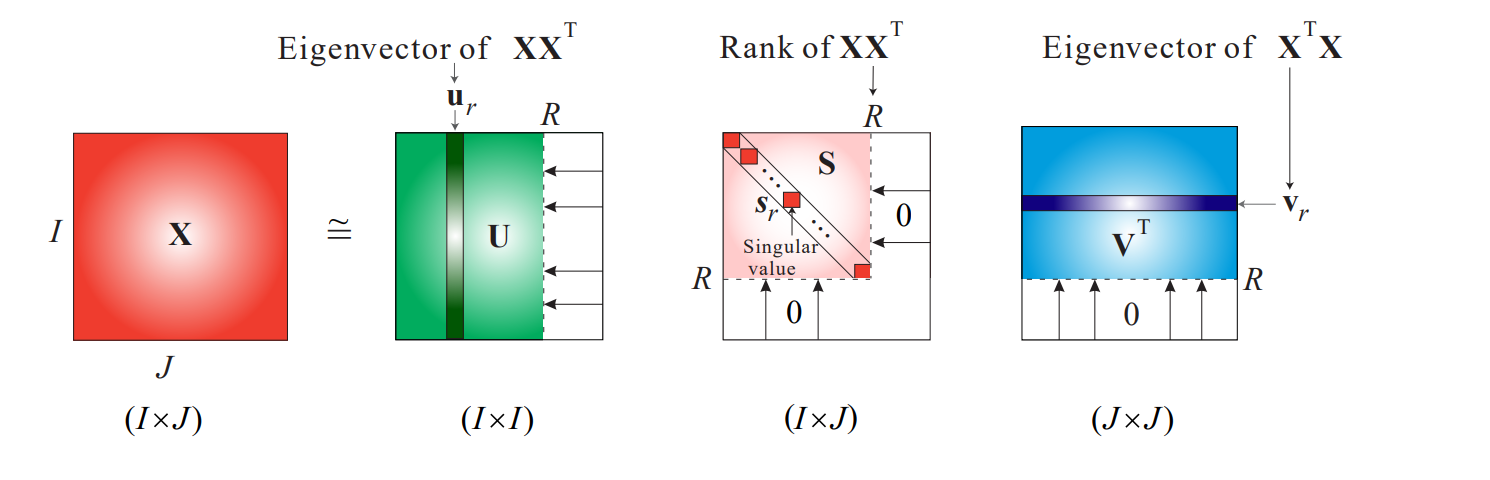
\includegraphics[width=0.9\textwidth]{lecture_12/figs/SVD.png}
\end{figure}
\end{frame}

%=======
\begin{frame}{Краткое повторение: HOSVD}
В случае тензоров можно применить ту же логику, как и в матричном SVD.\\
Любой тензор $\tensor{X} \in \mathbb{R}^{I_1 \times ...\times I_N}$ представляется в виде 
$$ \tensor{X}
= \llbracket \tensor{S}; \M{U}^{(1)}, ... ,\M{U}^{(d)}\rrbracket
$$
При этом:
\begin{itemize}
    \item $\M{U}^{(k)} \in \mathbb{R}^{n_k \times n_k}$ - ортогональные матрицы (factor matrices), условие аналогичное матричному SVD.
    \item В тензоре $\tensor{S}$  подтензоры $\tensor{S}_{:,...,:,i_n,:,...,:}$ имеют свойства:
    \begin{itemize}
        \item $\langle \tensor{S}_{:,...,:,i_n,:,...,:}\tensor{S}_{:,...,:,j_n,:,...,:}\rangle_F = 0$ для $i_n\neq j_n$, где $i_n,j_n \in \overline{1, I_n}$, то есть подтензоры, соответствующие разным индексам вдоль одной моды, взаимно ортогональны,
        \item $\lVert \tensor{S}_{:,...,:,i_n,:,...,:} \rVert_F \geq \lVert \tensor{S}_{:,...,:,j_n,:,...,:} \rVert_F \text{  при  } i_n \geq j_n$, где норма $\sigma_{i_n} :=  \lVert \tensor{S}_{:,...,:,i_n,:,...,:} \rVert_F$ -- это сингулярное число развёртки вдоль соответствующей моды $\tensor{S}_{(n)}$.
    \end{itemize}
\end{itemize}

\end{frame}
%=======
\begin{frame}{Краткое повторение: HOSVD}
\begin{figure}
    \centering
    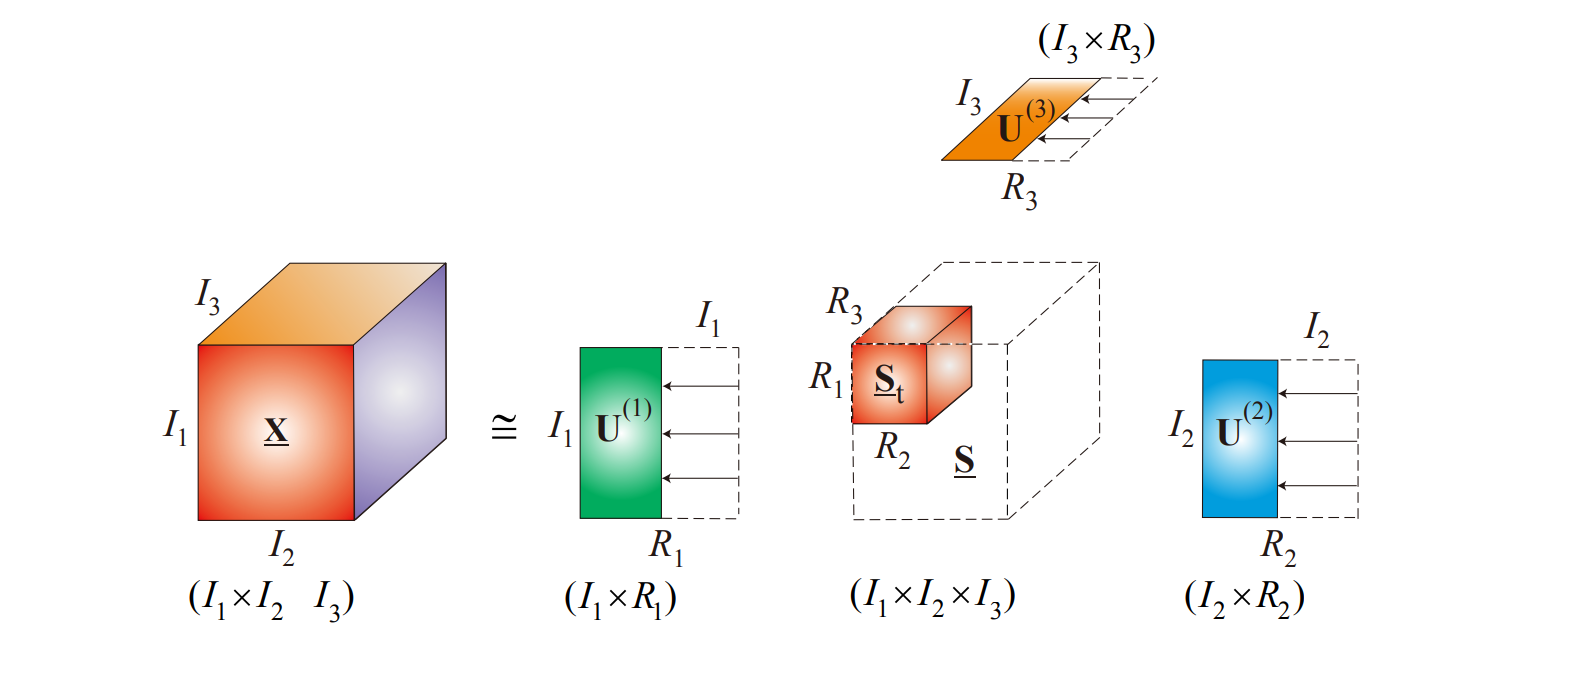
\includegraphics[width=1.1\textwidth]{lecture_12/figs/HOSVD.png}
\end{figure}
\end{frame}

%=======
\begin{frame}{Partial least squares regression}
Метод PLS позволяет выделить из исходных данных компоненты, между которыми существует
ковариационная связь.
\begin{itemize}
    \item Принцип метода PLS заключается в поиске общего набора скрытых переменных в независимой переменной $\M{X} \in \mathbb{R}^{I \times J}$ и зависимой переменной $\M{Y} \in \mathbb{R}^{I \times M}$ с помощью разложения.
    \item Компоненты, полученные в результате такого разложения, учитывают ковариацию между $\M{X}$ и $\M{Y}$.
\end{itemize}

\end{frame}
%=======
\begin{frame}{Partial least squares regression}
Задача заключается в том, чтобы представить матрицы $\M{X}$ и $\M{Y}$ в следующем виде:
\begin{equation*}
    \begin{split}
    \M{X} & = \M{T}\M{P}^{\intercal} + \M{E} = \sum_{r=1}^{R}\M{t}_r\M{p}_r^{\intercal} + \M{E}, \\
    \M{Y} & = \M{T}\M{D}\M{C}^{\intercal}+ \M{F} = \sum_{r=1}^{R}d_{rr}\M{t}_r\M{c}_r^{\intercal} + \M{F},
    \end{split}
\end{equation*}
где \begin{itemize}
    \item $\M{T} \in \mathbb{R}^{I \times R}$ матрица скрытых переменных из $\M{X}$,
    \item $\M{U} = \M{T}\M{D}$ матрица скрытых переменных из $\M{Y}$, имеющих наибольшую ковариацию с  $\M{T}$,
    \item $\M{D}$ --- диагональная масштабирующая матрица (линейное отображение),
    \item $\M{P}$ и $\M{C}$ --- матрицы весов,
    \item $\M{E}$ и $\M{F}$ --- регрессионные остатки
\end{itemize}    
\end{frame}
%=======
\begin{frame}{Partial least squares regression}
Стандартный алгоритм PLS:
\begin{itemize}
    \item находит два набора весовых векторов $\M{w}$ и $\M{c}$ с помощью следующей задачи оптимизации:
$$
\begin{aligned}[t]
    \underset{\{\M{w}, \M{c}\}}{\text{max}} & \quad (\M{w}^{\intercal}\M{X}^{\intercal}\M{Y}\M{c})^2,\\
    \text{s.t.} & \quad \M{w}^{\intercal}\M{w}=1,\quad \M{c}^{\intercal}\M{c}=1,
\end{aligned},
$$
\item искомые скрытые выражаются как $\M{t}=\frac{\M{X}\M{w}}{\norm{\M{X}\M{w}}_2^2}$ и $\M{u}=\M{Y}\M{c}$,
\item итерация повторяется пока не будет набрано желаемое число компонент.
\end{itemize} 
\end{frame}
%=======
\begin{frame}{Partial least squares regression}
\begin{figure}
    \centering
    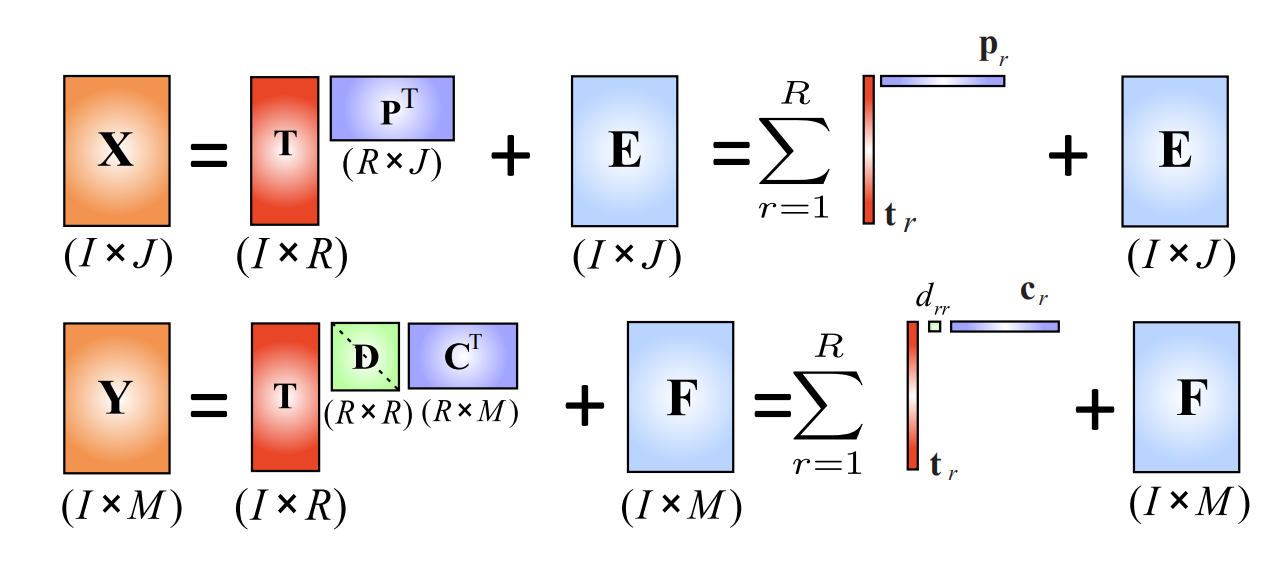
\includegraphics[width=1\textwidth]{lecture_13/figs/PLS_2D.png}
\end{figure}
\end{frame}
%=======
\begin{frame}{Higher-Order Partial Least Squares}
В случае тензоров, используя обобщенный HOSVD, можно применить ту же логику для PLS.\\
\begin{itemize}
    \item Обобщенная модель регрессии HOPLS выполняет одновременное разложение Такера с ограничениями для тензора с одинаковой размерностью первой моды, т.е. числа объектов в выборке.
    \item Предполагается, что $\tensor{X}$ разлагается как сумма блоков Такера ранга $(1, L_1,..., L_N)$, а  $\tensor{Y}$ разлагается как сумма блоков Такера ранга $(1, K_1,..., K_N)$, которые можно выразить как
\end{itemize}
 $$
\begin{aligned}[t]
    \tensor{X} &= \sum_{r=1}^{R}\textbf{G}_{xr}
    \times_1\M{t}_r
    \times_2\M{P}_r^{(1)}
    ...
    \times_{N+1}\M{P}_r^{(N)}
    + \tensor{E}_R\\
    \tensor{Y} &= \sum_{r=1}^{R}\textbf{G}_{yr}
    \times_1\M{t}_r
    \times_2\M{Q}_r^{(1)}
    ...
    \times_{N+1}\M{Q}_r^{(N)}
    + \tensor{F}_R.
\end{aligned}
 $$
\end{frame}

%=======
\begin{frame}{Higher-Order Partial Least Squares}
Модель HOPLS представима в виде:
 $$
\begin{aligned}[t]
    \tensor{X} &= \sum_{r=1}^{R}\textbf{G}_{xr}
    \times_1\M{t}_r
    \times_2\M{P}_r^{(1)}
    ...
    \times_{N+1}\M{P}_r^{(N)}
    + \tensor{E}_R\\
    \tensor{Y} &= \sum_{r=1}^{R}\textbf{G}_{yr}
    \times_1\M{t}_r
    \times_2\M{Q}_r^{(1)}
    ...
    \times_{N+1}\M{Q}_r^{(N)}
    + \tensor{F}_R.
\end{aligned}
 $$
где
\begin{itemize}
    \item $\M{t}_r \in \mathbb{R}^M$ --- векторы скрытых переменных по первой моде,
    \item $\{\M{P}_r^{(n)}\}_{n=1}^N \in \mathbb{R}^{I_n\times L_n} $ и $\{\M{Q}_r^{(n)}\}_{n=1}^N \in \mathbb{R}^{J_n\times K_n} $ --- фактор-матрицы по каждой моде,
    \item ${\tensor{G}_{x}}_r\in  \mathbb{R}^{1\times L_1\times...\times L_n}$ и ${\tensor{G}_{y}}_r\in  \mathbb{R}^{1\times K_1\times...\times K_n}$ --- центральные тензоры разложения
\end{itemize}
\end{frame}

%=======
\begin{frame}{Higher-Order Partial Least Squares}
\begin{figure}
    \centering
    \includegraphics[width=0.7\textwidth]{lecture_13/figs/HOPLS.png}
\end{figure}
\end{frame}
%=======
\begin{frame}{Partial least squares regression}
По аналогии сo стандартным алгоритмом PLS, в HOPLS:
\begin{itemize}
    \item находит два набора фактор-матриц $\M{P}^{(n)}_r$, $\M{Q}^{(n)}_r$ с помощью следующей задачи оптимизации:
$$
\begin{aligned}[t]
    \underset{\{\M{P}^{(n)}, \M{Q}^{(n)}\}}{\text{max}} & \llbracket \langle \tensor{X}, \tensor{Y} \rangle_{1;1}; \M{P}^{(1)},...,\M{P}^{(N)},\M{Q}^{(1)},...,\M{Q}^{(N)}\rrbracket,\\
    \text{s.t.} & \quad \M{P}^{(n)}^{\intercal}\M{P}^{(n)}=\M{I}_{L_n},\quad \M{Q}^{(n)}^{\intercal}\M{Q}^{(n)}=\M{I}_{K_n},
\end{aligned},
$$
\item Это эквивалентно нахождению наилучшего низкорангового приближения тензора $\langle \tensor{X}, \tensor{Y} \rangle_{1;1}$
\end{itemize} 
\end{frame}
%=======

\begin{frame}{Алгоритм Higher Order Partial Least Squares}

\textbf{Input:} тензоры $\tensor{X} \in \mathbb{R}^{M \times I_1 \times \dots \times I_N}$ и $\tensor{Y} \in \mathbb{R}^{M \times J_1 \times \dots \times J_N}$.  \\
\textbf{Output:} $\{ \M{P}_r^{(n)} \}$, $\{ \M{Q}_r^{(n)} \}$, $\{ {\tensor{G}_{x}}_r \}$, $\{ {\tensor{G}_{y}}_r \}$, $\M{T}$, $n = 1, \dots, N, \ r = 1, \dots, R$.

\begin{enumerate}
    \item \textbf{for} $r=1$ \textbf{to} $R$ \textbf{do}
    \item $\quad$ $\tensor{C} \leftarrow \langle \tensor{X}, \tensor{Y} \rangle_{1;1} \in \mathbb{R}^{I_1 \times \dots \times I_N \times J_1 \times \dots \times J_N}$.
    \item $\quad$ Найдём $\{ \M{P}_r^{(n)} \}$ и $\{ \M{Q}_r^{(n)} \}$ с помощью HOOI для $\tensor{C}$.
    \item $\quad$ $\M{t}_r \leftarrow \ $ синг. вектор $\Big(\tensor{X} \times_2 \M{P}_r^{(1)}^\intercal \times_3 \dots  \times_{N+1} \M{P}_r^{(N)}^\intercal \Big)_{(1)}$
    \item $\quad$ ${\tensor{G}_x}_r \leftarrow \tensor{X} \times_1 \M{t}_r^\intercal \times_2 \M{P}_r^{(1)}^\intercal \times_3 \dots  \times_{N+1} \M{P}_r^{(N)}^\intercal$
    \item $\quad$ ${\tensor{G}_y}_r \leftarrow \tensor{Y} \times_1 \M{t}_r^\intercal \times_2 \M{Q}_r^{(1)}^\intercal \times_3 \dots  \times_{N+1} \M{Q}_r^{(N)}^\intercal$
    \item $\quad$  $\tensor{X} \leftarrow \tensor{X} - {\tensor{G}_x}_r \times_1 \M{t}_r \times_2 \M{P}_r^{(1)} \times_3 \dots  \times_{N+1} \M{P}_r^{(N)}$
    \item $\quad$  $\tensor{Y} \leftarrow \tensor{Y} - {\tensor{G}_y}_r \times_1 \M{t}_r \times_2 \M{Q}_r^{(1)} \times_3 \dots  \times_{N+1} \M{Q}_r^{(N)}$
    \item \textbf{end for}
\end{enumerate}

\end{frame}

%=======

\begin{frame}{Пример HOPLS}
\begin{figure}
    \centering
    \includegraphics[width=0.6\textwidth]{lecture_10/figs/HOPLS.png}
\end{figure}
\begin{figure}
    \centering
    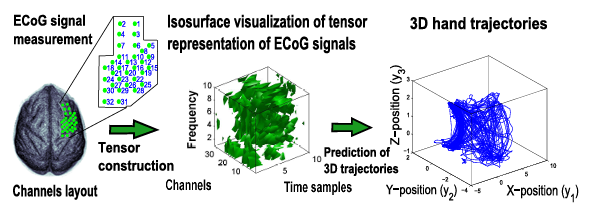
\includegraphics[width=0.6\textwidth]{lecture_10/figs/HOPLS_example.png}
\end{figure}

\end{frame}
%=======
\begin{frame}{Резюме}
\begin{itemize}
    \item PLS-регрессия --- это связанный с SVD статистический метод, который находит модель линейной регрессии, проецируя прогнозируемые переменные и наблюдаемые переменные в новое пространство.
    \item В новом пространстве выбираются скрытые переменные с наибольшей ковариацией. 
    \item По аналогии водится обобщение PLS --- HOPLS, основанный на разложении Такера.
    \item В этом разложении особую роль играет мода, соответствующая объектам выборки.
\end{itemize}
\end{frame}
\end{document} 